\documentclass[11pt,a4paper]{article}

\usepackage[a4paper,margin=2.5cm]{geometry}


\usepackage{amsmath,amssymb,amsthm}
\usepackage{booktabs}
\usepackage{tikz}
\usetikzlibrary{arrows.meta,positioning,shapes.geometric,fit,backgrounds,calc}
\usepackage{pgfplots}
\pgfplotsset{compat=1.18}
\usepackage[most]{tcolorbox}
\usepackage{hyperref}

\hypersetup{
    colorlinks=true,
    linkcolor=teal!80!black,
    citecolor=teal!80!black,
    urlcolor=teal!80!black
}

% -------------------------------------------------------------
% Mathematical Environments & Styling
% -------------------------------------------------------------
\theoremstyle{definition}
\newtheorem{definition}{Definition}[section]
\newtheorem{example}{Example}[section]
\newtheorem{algorithm}{Algorithm}[section]

\theoremstyle{plain}
\newtheorem{theorem}{Theorem}[section]
\newtheorem{lemma}{Lemma}[section]
\newtheorem{proposition}{Proposition}[section]
\newtheorem{corollary}{Corollary}[section]

% Custom Intuition Box (Blue tcolorbox)
\newtcolorbox{intuitionbox}[1][]{
    enhanced,
    colback=blue!5!white,
    colframe=blue!65!black,
    arc=3mm,
    boxrule=1pt,
    title=\textbf{Intuition: #1},
    coltitle=white,
    fonttitle=\bfseries,
    attach boxed title to top left={yshift=-2mm, xshift=4mm},
    boxed title style={colback=blue!65!black, arc=1.5mm},
    top=4mm,
    bottom=3mm,
    left=3mm,
    right=3mm,
    breakable
}

% Visual Blank Spot Box for Hard-to-Reproduce Slide Graphics
\newcommand{\slideimageplaceholder}[2]{
    \begin{center}
    \begin{tcolorbox}[
        enhanced,
        colback=gray!8!white,
        colframe=gray!60!black,
        width=0.92\textwidth,
        arc=2mm,
        frame hidden,
        borderline={0.5mm}{0mm}{gray!60!black, dashed},
        halign=center
    ]
        \vspace{0.4cm}
        \textbf{\textsf{[Visual Reference / Slide Artifact Placement]}} \\
        \vspace{0.2cm}
        \textsf{\textbf{Slide Source:} Slide #1} \\
        \textsf{\textbf{Suggested Caption:} #2}
        \vspace{0.4cm}
    \end{tcolorbox}
    \end{center}
}

\title{\textbf{\LARGE Neural Networks for Sequential Information Processing} \\ 
\Large Comprehensive Lecture Notes \& Mathematical Foundations}
\author{\textbf{Danilo Comminiello} \\ 
Department of Information Engineering, Electronics and Telecommunications \\ 
Sapienza University of Rome}
\date{Academic Year 2026/2027 --- November 10, 2026}

\begin{document}

\maketitle
\tableofcontents
\newpage

% =============================================================
\section{Sequence Data and Temporal Dependencies \emph{(slides 4--24)}}
% =============================================================

\subsection{Why Do We Need Sequence Models? \emph{(slides 4--5)}}
Traditional feedforward neural networks (e.g., standard Multi-Layer Perceptrons) implicitly treat distinct feature vectors as independent and identically distributed draws from a static underlying distribution. However, in physical, biological, linguistic, and financial environments, observations arrive in an ordered temporal continuum where \textbf{order carries essential predictive semantics}.

For example, consider natural language syntax: \emph{``dog bites man''} conveys an entirely different semantic event than \emph{``man bites dog''}, despite having identical token bags. Similar sequential properties dictate speech acoustics, bio-signals (ECG/EEG), and multi-sensor telemetry.

\begin{intuitionbox}[Feedforward Networks vs. Temporal Continuity]
A standard feedforward network is memoryless: if presented with input vector $\mathbf{x}_t$, it produces output $\mathbf{y}_t = f(\mathbf{x}_t; \boldsymbol{\theta})$ purely as a static function of that momentary snapshot. It does not possess internal inertial state variables that persist across $t-1$ to $t$. If we permute the temporal order of inputs fed one-by-one to an MLP, each individual output is completely unaffected, even though the sequential structure of the phenomenon has been destroyed.
\end{intuitionbox}

\subsection{Mathematical Representation of Sequences \emph{(slides 6--7)}}

\begin{definition}[Sequence Representation]
A multivariate sequence of duration $T$ is represented as an ordered tuple of column vectors:
\begin{equation}
    \mathbf{x}_{1:T} = (\mathbf{x}_1, \mathbf{x}_2, \dots, \mathbf{x}_T), \quad \text{where } \mathbf{x}_t \in \mathbb{R}^d.
\end{equation}
Here, $t \in \{1, \dots, T\}$ denotes the discrete sequence position, $d$ denotes the feature dimensionality, and $T$ is the total sequence length. When stacked as rows into a design matrix, we have:
\begin{equation}
    \mathbf{X} = \begin{bmatrix} \mathbf{x}_1^\top \\ \mathbf{x}_2^\top \\ \vdots \\ \mathbf{x}_T^\top \end{bmatrix} \in \mathbb{R}^{T \times d}.
\end{equation}
\end{definition}

\begin{figure}[htbp]
\centering
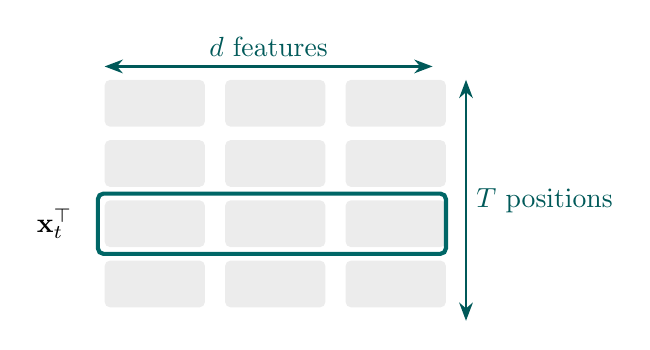
\begin{tikzpicture}[scale=0.85]
    \foreach \r in {0,1,2,3} {
        \foreach \c in {0,1,2} {
            \fill[fill=gray!15, rounded corners=2pt] (\c*1.8, -\r*0.9) rectangle ++(1.5, 0.7);
        }
    }
    % Highlight row t
    \draw[line width=1.5pt, draw=teal!80!black, rounded corners=2pt] (-0.1, -1.9) rectangle ++(5.2, 0.9);
    \node[left=0.2cm of {(-0.1, -1.45)}] {$\mathbf{x}_t^\top$};
    
    % Dimension markers
    \draw[<->, >=Stealth, thick, teal!70!black] (0, 0.9) -- ++(4.9, 0) node[midway, above] {$d \text{ features}$};
    \draw[<->, >=Stealth, thick, teal!70!black] (5.4, 0.7) -- ++(0, -3.6) node[midway, right] {$T \text{ positions}$};
\end{tikzpicture}
\caption{Matrix arrangement of a temporal sequence $\mathbf{X} \in \mathbb{R}^{T \times d}$.}
\end{figure}

For regularly sampled physical processes governed by a sampling period $\Delta t$, the continuous time coordinate is $t \cdot \Delta t$, corresponding to the sampling rate $f_s = \frac{1}{\Delta t}$. In stochastic modeling, the sequence is treated as a realization of an indexed stochastic process $\{\mathbf{X}_t\}_{t \in \mathcal{T}}$.

\subsection{Sequence Learning Tasks \emph{(slides 8--9)}}
Sequence learning configurations are categorized based on input and output cardinalities:
\begin{enumerate}
    \item \textbf{Sequence-to-Vector (Many-to-One):} Maps an entire sequence $\mathbf{x}_{1:T}$ to a single target $\mathbf{y} \in \mathbb{R}^q$ (e.g., sentiment classification, whole-utterance acoustic recognition).
    \item \textbf{Aligned Sequence-to-Sequence (Many-to-Many Aligned):} Maps an input sequence to an output sequence of equal length, producing target $\mathbf{y}_t$ synchronously at every position $t \in \{1, \dots, T\}$ (e.g., frame-level phoneme labeling, video tracking).
    \item \textbf{Autoregressive Prediction:} Predicts the subsequent value $\mathbf{x}_{t+1}$ conditioned upon the causal historical window $\mathbf{x}_{1:t}$.
    \item \textbf{Sequence Transduction (Many-to-Many Unaligned):} Maps an input sequence of length $T$ to an output sequence of length $U$ where $U \neq T$ in general (e.g., neural machine translation, speech-to-text).
\end{enumerate}

\subsection{Temporal Dependence and Statistical Characterization \emph{(slides 10--14)}}

\begin{definition}[Temporal Dependence]
A sequence exhibits temporal dependence if conditioning on past history modifies the conditional probability density/mass function of the current observation:
\begin{equation}
    p(\mathbf{x}_t \mid \mathbf{x}_{1:t-1}) \neq p(\mathbf{x}_t).
\end{equation}
Conversely, the sequence is temporally independent if and only if $p(\mathbf{x}_t \mid \mathbf{x}_{1:t-1}) = p(\mathbf{x}_t)$ for all $t$.
\end{definition}

For a multivariate process $\mathbf{X}_t \in \mathbb{R}^d$ with finite second moments, the mean vector is $\boldsymbol{\mu}_t = \mathbb{E}[\mathbf{X}_t]$, and the cross-covariance matrix function is defined as:
\begin{equation}
    \boldsymbol{\Gamma}(t, s) = \operatorname{Cov}(\mathbf{X}_t, \mathbf{X}_s) = \mathbb{E}\left[(\mathbf{X}_t - \boldsymbol{\mu}_t)(\mathbf{X}_s - \boldsymbol{\mu}_s)^\top\right] \in \mathbb{R}^{d \times d}.
\end{equation}

\begin{definition}[Weak-Sense Stationarity (WSS)]
A stochastic process $\{\mathbf{X}_t\}$ is weak-sense (wide-sense) stationary if:
\begin{enumerate}
    \item The mean is time-invariant: $\boldsymbol{\mu}_t = \boldsymbol{\mu} \in \mathbb{R}^d$ for all $t \in \mathcal{T}$.
    \item The covariance depends solely on the temporal lag $\tau = t - s$:
    \begin{equation}
        \boldsymbol{\Gamma}(t, s) = \boldsymbol{\Gamma}(t - s) = \boldsymbol{\Gamma}(\tau).
    \end{equation}
\end{enumerate}
For a scalar stationary process ($d=1$), the autocovariance is $\gamma(\tau) = \operatorname{Cov}(X_t, X_{t-\tau})$, and the normalized autocorrelation function (ACF) is:
\begin{equation}
    \rho(\tau) = \frac{\gamma(\tau)}{\gamma(0)}, \quad \text{with } \gamma(0) = \operatorname{Var}(X_t) > 0.
\end{equation}
\end{definition}

\begin{definition}[White Noise Process]
A scalar process $\{\epsilon_t\}$ is a (weak) white noise process, denoted $\epsilon_t \sim \operatorname{WN}(0, \sigma^2)$, if $\mathbb{E}[\epsilon_t] = 0$, $\operatorname{Var}(\epsilon_t) = \sigma^2 < \infty$, and $\operatorname{Cov}(\epsilon_t, \epsilon_s) = 0$ for all $t \neq s$.
\end{definition}

\begin{intuitionbox}[Linear Correlation vs. Nonlinear Dependence]
White noise only guarantees \emph{uncorrelatedness} ($\rho(\tau) = 0$ for $\tau \neq 0$), which measures absence of linear dependence. It does \textbf{not} imply statistical independence ($p(\epsilon_t, \epsilon_s) = p(\epsilon_t)p(\epsilon_s)$). For example, a process defined by $\epsilon_t = \eta_t \eta_{t-1}$ with i.i.d.\ zero-mean $\eta_t$ can be completely uncorrelated across non-zero lags, yet carries strong nonlinear deterministic dependencies that an MLP or RNN can exploit.
\end{intuitionbox}

\subsection{Classical Temporal Models: AR, MA, ARMA, ARIMA \emph{(slides 15--18)}}
Classical parametric time-series analysis formulates observations through linear stochastic difference equations driven by white-noise innovations $\epsilon_t$:

\begin{definition}[Autoregressive Process $\operatorname{AR}(p)$]
An autoregressive model of order $p$ regresses $x_t$ on its own past $p$ values:
\begin{equation}
    x_t = c + \sum_{i=1}^p a_i x_{t-i} + \epsilon_t,
\end{equation}
where $c$ is a constant intercept, $a_1, \dots, a_p \in \mathbb{R}$ are autoregressive coefficients, and $\epsilon_t \sim \operatorname{WN}(0, \sigma^2)$.
\end{definition}

\begin{definition}[Moving-Average Process $\operatorname{MA}(q)$]
A moving-average model of order $q$ models $x_t$ as a linear combination of current and past unobserved white-noise innovations:
\begin{equation}
    x_t = c + \epsilon_t + \sum_{j=1}^q b_j \epsilon_{t-j}.
\end{equation}
\end{definition}

\begin{definition}[Autoregressive Moving-Average Process $\operatorname{ARMA}(p, q)$]
Combining both dependency structures yields the $\operatorname{ARMA}(p, q)$ generator:
\begin{equation}
    x_t = c + \sum_{i=1}^p a_i x_{t-i} + \epsilon_t + \sum_{j=1}^q b_j \epsilon_{t-j}.
\end{equation}
Using the backshift (lag) operator $B$, where $B^k x_t = x_{t-k}$, this is written compactly as:
\begin{equation}
    \left(1 - \sum_{i=1}^p a_i B^i\right) x_t = c + \left(1 + \sum_{j=1}^q b_j B^j\right) \epsilon_t.
\end{equation}
\end{definition}

\begin{figure}[htbp]
\centering
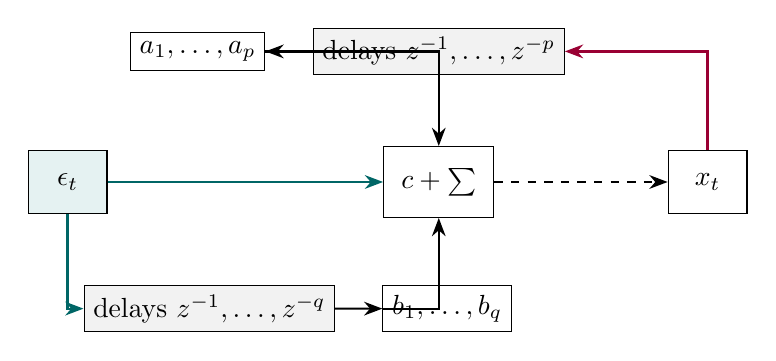
\begin{tikzpicture}[scale=0.85, auto, >=Stealth, node distance=1.3cm]
    \node (eps) [draw, rectangle, fill=teal!10, minimum height=0.8cm, minimum width=1cm] {$\epsilon_t$};
    \node (sum) [draw, rectangle, right=3.5cm of eps, minimum height=0.9cm, minimum width=1.4cm] {$c + \sum$};
    \node (out) [draw, rectangle, right=2.2cm of sum, minimum height=0.8cm, minimum width=1cm] {$x_t$};
    
    % Delays for AR
    \node (delay_ar) [draw, rectangle, above=0.9cm of sum, fill=gray!10] {delays $z^{-1}, \dots, z^{-p}$};
    \node (weights_ar) [draw, rectangle, left=0.6cm of delay_ar] {$a_1, \dots, a_p$};
    
    % Delays for MA
    \node (delay_ma) [draw, rectangle, below=0.9cm of eps, xshift=1.8cm, fill=gray!10] {delays $z^{-1}, \dots, z^{-q}$};
    \node (weights_ma) [draw, rectangle, right=0.6cm of delay_ma] {$b_1, \dots, b_q$};
    
    \draw[->, thick, teal!80!black] (eps) -- (sum);
    \draw[->, thick, dashed] (sum) -- (out);
    \draw[->, thick, purple!80!black] (out.north) |- (delay_ar.east);
    \draw[->, thick] (delay_ar) -- (weights_ar);
    \draw[->, thick] (weights_ar) -| (sum.north);
    
    \draw[->, thick, teal!80!black] (eps.south) |- (delay_ma.west);
    \draw[->, thick] (delay_ma) -- (weights_ma);
    \draw[->, thick] (weights_ma) -| (sum.south);
\end{tikzpicture}
\caption{Block diagram of an $\operatorname{ARMA}(p, q)$ generator with feedback of lagged observations and feedforward filtering of lagged innovations.}
\end{figure}

\begin{definition}[Autoregressive Integrated Moving Average $\operatorname{ARIMA}(p, d, q)$]
When a time-series is non-stationary in the mean (exhibiting stochastic trends), integration of order $d$ is applied via differencing:
\begin{equation}
    w_t = \Delta^d x_t = (1 - B)^d x_t, \quad d \in \{0, 1, 2, \dots\}.
\end{equation}
The differenced stationary series $w_t$ is then modeled via an $\operatorname{ARMA}(p, q)$ process.
\end{definition}

\subsection{Probabilistic Modeling and Learned Memory \emph{(slides 19--24)}}
From a rigorous probabilistic perspective, sequence prediction models the conditional distribution of future observations given historical observations: $p(\mathbf{x}_{t+1} \mid \mathbf{x}_{1:t})$.

\begin{theorem}[Autoregressive Factorization / Probability Chain Rule]
For any joint distribution over a sequence $\mathbf{x}_{1:T}$ admitting a probability density or mass function, the joint distribution factors \textbf{exactly} as:
\begin{equation}
    p(\mathbf{x}_{1:T}) = p(\mathbf{x}_1) \prod_{t=2}^T p(\mathbf{x}_t \mid \mathbf{x}_{1:t-1}).
\end{equation}
This holds identically without requiring any stationarity, linearity, or Markov assumptions.
\end{theorem}

\begin{definition}[Markov Assumption of Order $p$]
Under an exact Markov assumption of order $p$, the conditional distribution truncates historical dependency strictly to the preceding $p$ steps:
\begin{equation}
    p(\mathbf{x}_t \mid \mathbf{x}_{1:t-1}) = p(\mathbf{x}_t \mid \mathbf{x}_{t-p:t-1}).
\end{equation}
\end{definition}

\begin{intuitionbox}[Fixed External Buffers vs. Evolving Hidden States]
To build a neural sequence model, we face a fundamental design fork:
\begin{itemize}
    \item \textbf{Fixed Buffer (Feedforward MLP):} We assume a Markov order $p$. An explicit tapped delay line buffers $(\mathbf{x}_{t-p+1}, \dots, \mathbf{x}_t) \in \mathbb{R}^{pd}$. The network is static; history beyond horizon $p$ is permanently dropped.
    \item \textbf{Recurrent State (RNN):} Instead of storing raw observations in an expanding buffer, the network compresses all past history $\mathbf{x}_{1:t}$ into a fixed-dimensional dynamical state vector $\mathbf{h}_t \in \mathbb{R}^m$ via a learned state update $\mathbf{h}_t = f_{\boldsymbol{\theta}_h}(\mathbf{h}_{t-1}, \mathbf{x}_t)$.
\end{itemize}
\end{intuitionbox}

% =============================================================
\section{Neural Networks for Time-Series Prediction \emph{(slides 25--42)}}
% =============================================================

\subsection{Prediction Objectives \& Formal Problem Formulations \emph{(slides 25--26)}}
Time-series analysis decomposes into three distinct task archetypes governed by causality and information availability:
\begin{enumerate}
    \item \textbf{Forecasting (Prediction):} Given observed history up to forecast origin $t$, estimate future values:
    \begin{equation}
        \hat{\mathbf{x}}_{t+k \mid t} = f_{\boldsymbol{\theta}}(\mathbf{x}_{1:t}), \quad k \ge 1.
    \end{equation}
    Under squared error loss $\mathbb{E}[\|\mathbf{X}_{t+1} - \hat{\mathbf{x}}_{t+1}\|^2 \mid \mathbf{X}_{1:t} = \mathbf{x}_{1:t}]$, the Bayes-optimal point predictor is the conditional expectation:
    \begin{equation}
        \hat{\mathbf{x}}_{t+1}^* = \mathbb{E}[\mathbf{X}_{t+1} \mid \mathbf{X}_{1:t} = \mathbf{x}_{1:t}].
    \end{equation}
    \item \textbf{Filtering / Real-Time Estimation:} Given noisy observations up to time $t$, estimate a latent physical system state $\mathbf{s}_t$ using only causal information $\mathbf{x}_{1:t}$.
    \item \textbf{Smoothing / Retrospective Labeling (Offline):} In non-causal offline analysis, observations after time $t$ are known. The target is conditioned on the entire bilateral sequence: $p(\mathbf{y}_t \mid \mathbf{x}_{1:T})$.
\end{enumerate}

\subsection{Fixed-Context Buffered MLP Predictors \emph{(slides 27--30)}}
Given a scalar time series $\{x_t\}_{t=1}^N$, a sliding window of length $p$ forms feature vectors:
\begin{equation}
    \mathbf{v}_t = [x_{t-p+1}, x_{t-p+2}, \dots, x_t]^\top \in \mathbb{R}^p, \quad \text{with label } y_t = x_{t+1}.
\end{equation}
A feedforward Multi-Layer Perceptron parameterizes the nonlinear mapping:
\begin{equation}
    \hat{x}_{t+1} = f_{\boldsymbol{\theta}_{\text{MLP}}}(\mathbf{v}_t) = \mathbf{W}_2 \operatorname{ReLU}(\mathbf{W}_1 \mathbf{v}_t + \mathbf{b}_1) + b_2.
\end{equation}
Optimization minimizes the empirical Mean Squared Error (MSE) over the chronological training index set $\mathcal{I}_{\text{train}}$:
\begin{equation}
    \mathcal{L}(\boldsymbol{\theta}_{\text{MLP}}) = \frac{1}{|\mathcal{I}_{\text{train}}|} \sum_{t \in \mathcal{I}_{\text{train}}} (x_{t+1} - f_{\boldsymbol{\theta}_{\text{MLP}}}(\mathbf{v}_t))^2.
\end{equation}

\slideimageplaceholder{27 \& 30}{Synthetic noisy sinusoid dataset $x_t = \sin(0.03t) + 0.2\epsilon_t$ and corresponding one-step-ahead MLP predictions tracking the underlying smooth trend.}

\subsection{Multi-Step Forecasting: Recursive vs. Direct \emph{(slides 31--32)}}
Predicting $K$ steps into the future $\mathbf{x}_{t+1:t+K}$ can be accomplished via two fundamentally distinct strategies:

\begin{definition}[Recursive Multi-Step Forecasting]
Uses a single one-step-ahead model $f_{\boldsymbol{\theta}}$ iteratively. Predictions are fed back as synthetic inputs for subsequent predictions:
\begin{equation}
    \hat{x}_{t+k \mid t} = f_{\boldsymbol{\theta}}(\tilde{x}_{t+k-p}, \dots, \tilde{x}_{t+k-1}), \quad k = 1, \dots, K,
\end{equation}
where:
\begin{equation}
    \tilde{x}_j = \begin{cases} x_j, & j \le t \text{ (true observed sample)}, \\ \hat{x}_{j \mid t}, & j > t \text{ (previously predicted value)}. \end{cases}
\end{equation}
\end{definition}

\begin{definition}[Direct Multi-Step Forecasting]
Trains $K$ separate models $\{f_{\boldsymbol{\theta}_k}\}_{k=1}^K$ (or a joint vector-output network $\mathbf{F}_{\boldsymbol{\theta}_{\text{dir}}}$) to predict each horizon directly from historical observations alone:
\begin{equation}
    \hat{x}_{t+k \mid t} = f_{\boldsymbol{\theta}_k}(x_{t-p+1}, \dots, x_t), \quad \text{or} \quad [\hat{x}_{t+1 \mid t}, \dots, \hat{x}_{t+K \mid t}]^\top = \mathbf{F}_{\boldsymbol{\theta}_{\text{dir}}}(\mathbf{v}_t).
\end{equation}
\end{definition}

\begin{intuitionbox}[The Compounding Error Cascade in Autoregressive Rollouts]
In recursive forecasting, any error $|\hat{x}_{t+1} - x_{t+1}|$ corrupts the input buffer for $\hat{x}_{t+2}$. As the horizon $k$ increases, the network operates on inputs drawn from its own model distribution rather than the true data-generating distribution (\emph{exposure bias}). Consequently, predictions degrade rapidly and often collapse toward trivial mean values or divergent limit cycles. Direct forecasting prevents error propagation across steps, but sacrifices temporal consistency across neighboring prediction horizons.
\end{intuitionbox}

\slideimageplaceholder{32}{Degradation of recursive predictions across horizons $k \in \{1, 4, 16, 64\}$ on the noisy sinusoidal benchmark.}

\subsection{Nonlinear System Identification: NARX Architectures \emph{(slides 33--42)}}
In control and dynamical systems, the goal is often identifying an unknown plant driven by an external input $\{u_t\}$:

\begin{definition}[NARX: Nonlinear Autoregressive with Exogenous Inputs]
The output $\hat{y}_t$ is modeled as a nonlinear function of $p$ lagged outputs and $q+1$ input terms (current and $q$ lags):
\begin{equation}
    \hat{y}_t = f_{\boldsymbol{\theta}_{\text{NARX}}}(y_{t-1}, y_{t-2}, \dots, y_{t-p}, u_t, u_{t-1}, \dots, u_{t-q}).
\end{equation}
\end{definition}

Operating regimes for NARX models:
\begin{itemize}
    \item \textbf{Series-Parallel (Open-Loop / One-Step):} True system outputs $y_{t-1}, \dots, y_{t-p}$ are fed to the model at each step. The prediction error is:
    \begin{equation}
        e_t^{\text{pred}} = y_t - f_{\boldsymbol{\theta}}(y_{t-1:t-p}, u_{t:t-q}).
    \end{equation}
    \item \textbf{Parallel (Closed-Loop / Free-Running Simulation):} Model-generated outputs $\tilde{y}_{t-1}, \dots, \tilde{y}_{t-p}$ are fed back autonomously:
    \begin{equation}
        \tilde{y}_t = f_{\boldsymbol{\theta}}(\tilde{y}_{t-1:t-p}, u_{t:t-q}), \quad e_t^{\text{sim}} = y_t - \tilde{y}_t.
    \end{equation}
\end{itemize}

\slideimageplaceholder{39 \& 42}{System identification diagrams and free-running test simulation trajectories for the nonlinear benchmark $y_t = 0.6y_{t-1} + 0.2\tanh(2u_t) + 0.1u_{t-1}^2$.}

% =============================================================
\section{Recurrent Neural Networks \emph{(slides 43--71)}}
% =============================================================

\subsection{Representations and Dynamical Hidden States \emph{(slides 43--47)}}
Feedforward autoencoders map an input $\mathbf{x}$ to a spatial latent code $\mathbf{z} = f_{\text{enc}}(\mathbf{x})$ that discards task-irrelevant variations. In temporal learning, a recurrent hidden state $\mathbf{h}_t \in \mathbb{R}^m$ generalizes this concept to dynamic sequences:
\begin{equation}
    \mathbf{h}_t = f_{\boldsymbol{\theta}_h}(\mathbf{h}_{t-1}, \mathbf{x}_t), \quad \hat{\mathbf{y}}_t = g_{\boldsymbol{\theta}_o}(\mathbf{h}_t).
\end{equation}
Thus, $\mathbf{h}_t$ serves as a \textbf{deterministic lossy summary} of the arbitrary-length historical sequence $\mathbf{x}_{1:t}$.

\subsection{The Vanilla Elman Recurrent Neural Network \emph{(slides 48--54)}}

\begin{definition}[Elman RNN Equations]
For input vector $\mathbf{x}_t \in \mathbb{R}^d$ and previous hidden state $\mathbf{h}_{t-1} \in \mathbb{R}^m$, the forward equations of a standard Elman cell are:
\begin{align}
    \mathbf{a}_t &= \mathbf{W}_x \mathbf{x}_t + \mathbf{W}_h \mathbf{h}_{t-1} + \mathbf{b}_h, \label{eq:rnn_preact} \\
    \mathbf{h}_t &= \phi(\mathbf{a}_t), \label{eq:rnn_state} \\
    \mathbf{o}_t &= \mathbf{W}_y \mathbf{h}_t + \mathbf{b}_y, \label{eq:rnn_output}
\end{align}
where $\phi(\cdot)$ is an elementwise non-linear activation (typically $\tanh$), and the parameter matrices and vectors are:
\begin{equation}
    \mathbf{W}_x \in \mathbb{R}^{m \times d}, \quad \mathbf{W}_h \in \mathbb{R}^{m \times m}, \quad \mathbf{b}_h \in \mathbb{R}^m, \quad \mathbf{W}_y \in \mathbb{R}^{q \times m}, \quad \mathbf{b}_y \in \mathbb{R}^q.
\end{equation}
\end{definition}

\begin{figure}[htbp]
\centering
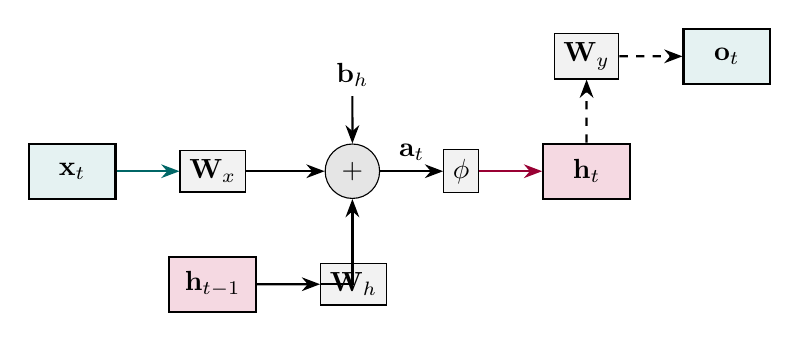
\begin{tikzpicture}[scale=0.9, auto, >=Stealth]
    \node (xt) [draw, rectangle, fill=teal!10, thick, minimum width=1.1cm, minimum height=0.7cm] {$\mathbf{x}_t$};
    \node (Wx) [draw, rectangle, fill=gray!10, right=0.8cm of xt] {$\mathbf{W}_x$};
    \node (sum) [draw, circle, fill=gray!20, right=1.0cm of Wx] {$+$};
    \node (bh) [above=0.6cm of sum] {$\mathbf{b}_h$};
    \node (phi) [draw, rectangle, fill=gray!10, right=0.8cm of sum] {$\phi$};
    \node (ht) [draw, rectangle, fill=purple!15, thick, right=0.8cm of phi, minimum width=1.1cm, minimum height=0.7cm] {$\mathbf{h}_t$};
    \node (Wy) [draw, rectangle, fill=gray!10, above=0.8cm of ht] {$\mathbf{W}_y$};
    \node (ot) [draw, rectangle, fill=teal!10, thick, right=0.8cm of Wy, minimum width=1.1cm, minimum height=0.7cm] {$\mathbf{o}_t$};
    
    \node (htm1) [draw, rectangle, fill=purple!15, thick, below=0.8cm of Wx, minimum width=1.1cm, minimum height=0.7cm] {$\mathbf{h}_{t-1}$};
    \node (Wh) [draw, rectangle, fill=gray!10, right=0.8cm of htm1] {$\mathbf{W}_h$};

    \draw[->, thick, teal!80!black] (xt) -- (Wx);
    \draw[->, thick] (Wx) -- (sum);
    \draw[->, thick] (bh) -- (sum);
    \draw[->, thick] (htm1) -- (Wh);
    \draw[->, thick] (Wh) -| (sum);
    \draw[->, thick] (sum) -- node[above] {$\mathbf{a}_t$} (phi);
    \draw[->, thick, purple!80!black] (phi) -- (ht);
    \draw[->, thick, dashed] (ht) -- (Wy);
    \draw[->, thick, dashed] (Wy) -- (ot);
\end{tikzpicture}
\caption{Detailed architectural graph of the Elman recurrent cell.}
\end{figure}

\begin{proposition}[Total Parameter Complexity of Vanilla RNN]
The total count of trainable parameters $N_{\text{par}}$ in an Elman RNN layer with input dimension $d$, hidden state dimension $m$, and output dimension $q$ is:
\begin{equation}
    N_{\text{par}} = \underbrace{m d}_{\mathbf{W}_x} + \underbrace{m^2}_{\mathbf{W}_h} + \underbrace{m}_{\mathbf{b}_h} + \underbrace{q m}_{\mathbf{W}_y} + \underbrace{q}_{\mathbf{b}_y} = m(d + m + 1) + q(m + 1).
\end{equation}
Critically, $N_{\text{par}}$ is \textbf{strictly independent} of sequence length $T$.
\end{proposition}

\begin{example}[Worked Parameter Calculation \emph{(slide 56)}]
For the sunspot univariate forecasting model where $d = 1$, $m = 28$ hidden recurrent units, and $q = 1$ output target:
\begin{align*}
    N_{\text{par}} &= 28(1 + 28 + 1) + 1(28 + 1) \\
    &= 28(30) + 29 = 840 + 29 = \mathbf{869} \text{ parameters}.
\end{align*}
\end{example}

\subsection{Elman vs. Jordan Recurrent Feedback \emph{(slide 53)}}
Two early recurrent topologies differ in the nature of their feedback loop:
\begin{itemize}
    \item \textbf{Elman Network (Hidden-to-Hidden):} Memory resides in internal representations:
    \begin{equation}
        \mathbf{h}_t = \phi(\mathbf{W}_x \mathbf{x}_t + \mathbf{W}_h \mathbf{h}_{t-1} + \mathbf{b}_h).
    \end{equation}
    \item \textbf{Jordan Network (Output-to-Hidden):} Memory resides in predictions fed back through context units $\mathbf{c}_t$:
    \begin{equation}
        \mathbf{h}_t = \phi(\mathbf{V}_x \mathbf{x}_t + \mathbf{V}_c \mathbf{c}_{t-1} + \mathbf{b}_J), \quad \text{where } \mathbf{c}_t = \lambda \mathbf{c}_{t-1} + \hat{\mathbf{y}}_t, \quad 0 \le \lambda < 1.
    \end{equation}
\end{itemize}

\subsection{Unfolding Through Time \& Shared Computation \emph{(slides 55--58)}}
A recurrent network with feedback delay $z^{-1}$ can be represented as an equivalent directed acyclic graph (DAG) by \textbf{unfolding} across sequence steps $t = 1, \dots, T$.

\begin{figure}[htbp]
\centering
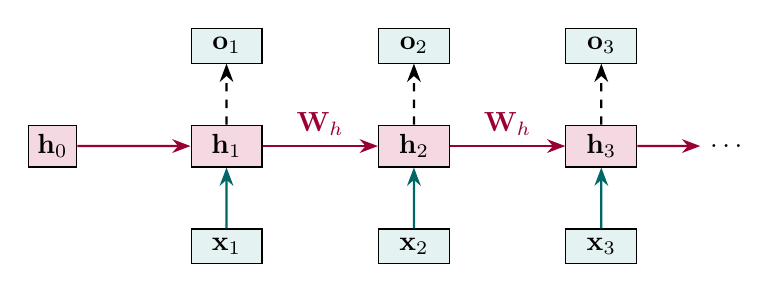
\begin{tikzpicture}[scale=0.85, auto, >=Stealth]
    \foreach \t/\x in {1/1, 2/2, 3/3} {
        \node (x\t) at (\t*2.8, 0) [draw, rectangle, fill=teal!10, minimum width=0.9cm] {$\mathbf{x}_{\t}$};
        \node (h\t) at (\t*2.8, 1.5) [draw, rectangle, fill=purple!15, minimum width=0.9cm] {$\mathbf{h}_{\t}$};
        \node (o\t) at (\t*2.8, 3.0) [draw, rectangle, fill=teal!10, minimum width=0.9cm] {$\mathbf{o}_{\t}$};
        \draw[->, thick, teal!80!black] (x\t) -- (h\t);
        \draw[->, thick, dashed] (h\t) -- (o\t);
    }
    \node (h0) at (0.2, 1.5) [draw, rectangle, fill=purple!15] {$\mathbf{h}_0$};
    \draw[->, thick, purple!80!black] (h0) -- (h1);
    \draw[->, thick, purple!80!black] (h1) -- node[above] {$\mathbf{W}_h$} (h2);
    \draw[->, thick, purple!80!black] (h2) -- node[above] {$\mathbf{W}_h$} (h3);
    \node (hdots) [right=0.8cm of h3] {$\dots$};
    \draw[->, thick, purple!80!black] (h3) -- (hdots);
\end{tikzpicture}
\caption{The computational graph of a recurrent neural network unfolded across time steps.}
\end{figure}

\begin{intuitionbox}[Unfolding Does Not Create New Parameters]
Unfolding is not a structural expansion of model parameters. The model has only one matrix $\mathbf{W}_x$, one matrix $\mathbf{W}_h$, and one matrix $\mathbf{W}_y$. Unfolding represents the dynamic dataflow of operations during execution. Every temporal slice is bound to the exact same parameter tensors.
\end{intuitionbox}

\subsection{Windowed vs. Stateful Recurrent Inference \emph{(slides 60--64)}}
When processing long or streaming data, execution splits into two distinct modes:
\begin{itemize}
    \item \textbf{Windowed Inference:} Given sequence chunks of length $T_w$, the hidden state is initialized to a constant vector (e.g., $\mathbf{h}_0 = \mathbf{0}$) at the start of \emph{every} window. The network cannot access any history that occurred prior to the current window boundary.
    \item \textbf{Stateful Inference:} The final hidden state of chunk $k$, $\mathbf{h}_{T_w}^{(k)}$, is carried forward as the initial state $\mathbf{h}_0^{(k+1)}$ for chunk $k+1$. Memory flows across boundaries while causal isolation is preserved. State resets occur only at true independent sequence boundaries.
\end{itemize}

\slideimageplaceholder{67 \& 68}{Synthetic controlled memory task ($s_t = 0.97s_{t-1} + 0.03x_t$): test RMSE comparison showing stateful RNN outperforming short-buffered MLP ($p=8$), and buffer scaling behavior up to $p=128$.}

% =============================================================
\section{Training Recurrent Neural Networks \emph{(slides 72--87)}}
% =============================================================

\subsection{Backpropagation Through Time (BPTT) Derivation \emph{(slides 72--78)}}
Consider a sequence of length $T$ with loss defined as the sum of step-wise scalar losses:
\begin{equation}
    \mathcal{L} = \sum_{t=1}^T \ell_t(o_t, y_t).
\end{equation}

\begin{theorem}[BPTT Exact Gradient Recursion]
Let $\mathbf{e}_t = \nabla_{\mathbf{o}_t} \ell_t \in \mathbb{R}^q$ denote the local error at the output layer. Define the hidden preactivation error adjoint vector as:
\begin{equation}
    \boldsymbol{\delta}_t \triangleq \nabla_{\mathbf{a}_t} \mathcal{L} \in \mathbb{R}^m.
\end{equation}
Then, the error adjoints obey the reverse-time backward recurrence:
\begin{equation}
    \boldsymbol{\delta}_t = \operatorname{diag}\left(\phi'(\mathbf{a}_t)\right) \left[ \mathbf{W}_y^\top \mathbf{e}_t + \mathbf{W}_h^\top \boldsymbol{\delta}_{t+1} \right], \quad \text{for } t = T, T-1, \dots, 1,
\end{equation}
initialized with the boundary condition $\boldsymbol{\delta}_{T+1} = \mathbf{0}$.
\end{theorem}

\begin{proof}
By the multivariable chain rule, the gradient of the total loss $\mathcal{L}$ with respect to the hidden state vector $\mathbf{h}_t$ receives two contributions: the direct local path from the current loss $\ell_t$, and the delayed path from the subsequent state $\mathbf{h}_{t+1}$:
\begin{align}
    \nabla_{\mathbf{h}_t} \mathcal{L} &= \left( \frac{\partial \mathbf{o}_t}{\partial \mathbf{h}_t} \right)^\top \nabla_{\mathbf{o}_t} \ell_t + \left( \frac{\partial \mathbf{a}_{t+1}}{\partial \mathbf{h}_t} \right)^\top \nabla_{\mathbf{a}_{t+1}} \mathcal{L} \\
    &= \mathbf{W}_y^\top \mathbf{e}_t + \mathbf{W}_h^\top \boldsymbol{\delta}_{t+1}.
\end{align}
Because $\mathbf{h}_t = \phi(\mathbf{a}_t)$, the Jacobian of the elementwise mapping is $\frac{\partial \mathbf{h}_t}{\partial \mathbf{a}_t} = \operatorname{diag}(\phi'(\mathbf{a}_t))$. Hence:
\begin{align}
    \boldsymbol{\delta}_t = \left( \frac{\partial \mathbf{h}_t}{\partial \mathbf{a}_t} \right)^\top \nabla_{\mathbf{h}_t} \mathcal{L} = \operatorname{diag}\left(\phi'(\mathbf{a}_t)\right) \left[ \mathbf{W}_y^\top \mathbf{e}_t + \mathbf{W}_h^\top \boldsymbol{\delta}_{t+1} \right].
\end{align}
\end{proof}

\begin{corollary}[Shared Parameter Gradients]
Since parameters $\mathbf{W}_h$, $\mathbf{W}_x$, $\mathbf{b}_h$, $\mathbf{W}_y$, and $\mathbf{b}_y$ are reused at every time step $t$, their total gradients are obtained by summing the outer products over all unrolled steps:
\begin{align}
    \nabla_{\mathbf{W}_h} \mathcal{L} &= \sum_{t=1}^T \boldsymbol{\delta}_t \mathbf{h}_{t-1}^\top \in \mathbb{R}^{m \times m}, \label{eq:grad_wh} \\
    \nabla_{\mathbf{W}_x} \mathcal{L} &= \sum_{t=1}^T \boldsymbol{\delta}_t \mathbf{x}_t^\top \in \mathbb{R}^{m \times d}, \label{eq:grad_wx} \\
    \nabla_{\mathbf{b}_h} \mathcal{L} &= \sum_{t=1}^T \boldsymbol{\delta}_t \in \mathbb{R}^m, \label{eq:grad_bh} \\
    \nabla_{\mathbf{W}_y} \mathcal{L} &= \sum_{t=1}^T \mathbf{e}_t \mathbf{h}_t^\top \in \mathbb{R}^{q \times m}, \quad \nabla_{\mathbf{b}_y} \mathcal{L} = \sum_{t=1}^T \mathbf{e}_t \in \mathbb{R}^q. \label{eq:grad_out}
\end{align}
\end{corollary}

\begin{figure}[htbp]
\centering
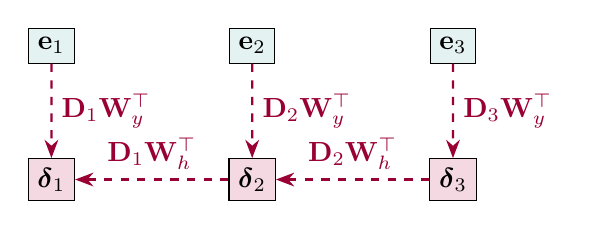
\begin{tikzpicture}[scale=0.85, auto, >=Stealth]
    \node (e1) at (2.5, 2.5) [draw, rectangle, fill=teal!10] {$\mathbf{e}_1$};
    \node (e2) at (5.5, 2.5) [draw, rectangle, fill=teal!10] {$\mathbf{e}_2$};
    \node (e3) at (8.5, 2.5) [draw, rectangle, fill=teal!10] {$\mathbf{e}_3$};
    
    \node (d1) at (2.5, 0.5) [draw, rectangle, fill=purple!15] {$\boldsymbol{\delta}_1$};
    \node (d2) at (5.5, 0.5) [draw, rectangle, fill=purple!15] {$\boldsymbol{\delta}_2$};
    \node (d3) at (8.5, 0.5) [draw, rectangle, fill=purple!15] {$\boldsymbol{\delta}_3$};
    
    \draw[->, thick, dashed, purple!80!black] (e3) -- node[right] {$\mathbf{D}_3 \mathbf{W}_y^\top$} (d3);
    \draw[->, thick, dashed, purple!80!black] (e2) -- node[right] {$\mathbf{D}_2 \mathbf{W}_y^\top$} (d2);
    \draw[->, thick, dashed, purple!80!black] (e1) -- node[right] {$\mathbf{D}_1 \mathbf{W}_y^\top$} (d1);
    
    \draw[->, thick, dashed, purple!80!black] (d3) -- node[above] {$\mathbf{D}_2 \mathbf{W}_h^\top$} (d2);
    \draw[->, thick, dashed, purple!80!black] (d2) -- node[above] {$\mathbf{D}_1 \mathbf{W}_h^\top$} (d1);
\end{tikzpicture}
\caption{The BPTT backward computational graph showing reverse-time propagation of adjoint errors, where $\mathbf{D}_t = \operatorname{diag}(\phi'(\mathbf{a}_t))$.}
\end{figure}

\subsection{Temporal Jacobians, Vanishing \& Exploding Gradients \emph{(slides 79--83)}}

\begin{definition}[Temporal State Jacobian]
The sensitivity of hidden state $\mathbf{h}_t$ to the previous state $\mathbf{h}_{t-1}$ is described by the temporal Jacobian matrix:
\begin{equation}
    \mathbf{J}_t \triangleq \frac{\partial \mathbf{h}_t}{\partial \mathbf{h}_{t-1}} = \operatorname{diag}\left(\phi'(\mathbf{a}_t)\right) \mathbf{W}_h \in \mathbb{R}^{m \times m}.
\end{equation}
By repeated application of the chain rule across an interval $k = t - s$ steps:
\begin{equation}
    \frac{\partial \mathbf{h}_t}{\partial \mathbf{h}_s} = \prod_{j=s+1}^t \mathbf{J}_j = \mathbf{J}_t \mathbf{J}_{t-1} \cdots \mathbf{J}_{s+1}.
\end{equation}
Consequently, the gradient of a distant loss $\ell_t$ with respect to state $\mathbf{h}_s$ is:
\begin{equation}
    \nabla_{\mathbf{h}_s} \ell_t = \left( \prod_{j=s+1}^t \mathbf{J}_j \right)^\top \nabla_{\mathbf{h}_t} \ell_t.
\end{equation}
\end{definition}

\begin{theorem}[Sufficient Condition for Vanishing Gradients]
Let $\|\cdot\|_2$ denote the spectral matrix norm. If there exists a constant $\gamma < 1$ such that for all $j$,
\begin{equation}
    \|\mathbf{J}_j\|_2 \le \gamma < 1,
\end{equation}
then the norm of the propagated gradient decays exponentially with temporal distance $k = t - s$:
\begin{equation}
    \left\| \nabla_{\mathbf{h}_s} \ell_t \right\|_2 \le \gamma^{t-s} \left\| \nabla_{\mathbf{h}_t} \ell_t \right\|_2 \xrightarrow{t-s \to \infty} 0.
\end{equation}
\end{theorem}

\begin{proof}
Applying the sub-multiplicative property of induced matrix norms:
\begin{equation}
    \left\| \prod_{j=s+1}^t \mathbf{J}_j^\top \right\|_2 \le \prod_{j=s+1}^t \|\mathbf{J}_j^\top\|_2 = \prod_{j=s+1}^t \|\mathbf{J}_j\|_2 \le \prod_{j=s+1}^t \gamma = \gamma^{t-s}.
\end{equation}
Multiplying by $\|\nabla_{\mathbf{h}_t} \ell_t\|_2$ yields the stated upper bound.
\end{proof}

\begin{intuitionbox}[The Geometric Mechanism of Vanishing and Exploding Gradients]
Consider the $\tanh(x)$ activation function. Its derivative is $\phi'(x) = 1 - \tanh^2(x) \in (0, 1]$.
\begin{itemize}
    \item \textbf{Vanishing Gradients:} If the largest singular value $\sigma_{\max}(\mathbf{W}_h) < 1$, then because $|\phi'| \le 1$, every Jacobian factor strictly contracts vectors: $\|\mathbf{J}_j\|_2 < 1$. Compounding 50 steps contracts gradients by at least $(0.9)^{50} \approx 0.00515$. Furthermore, if neurons saturate ($|a_t| \gg 0$), $\phi'(a_t) \to 0$, immediately destroying gradient flow regardless of $\mathbf{W}_h$.
    \item \textbf{Exploding Gradients:} If $\sigma_{\max}(\mathbf{W}_h) > 1$ and states remain in the linear regime of $\tanh$ ($\phi' \approx 1$), the product can amplify components along the dominant eigenvector exponentially: $(1.1)^{50} \approx 117.4$. This triggers catastrophic overflow (NaNs) or wild optimizer jumps.
\end{itemize}
\end{intuitionbox}

\begin{figure}[htbp]
\centering
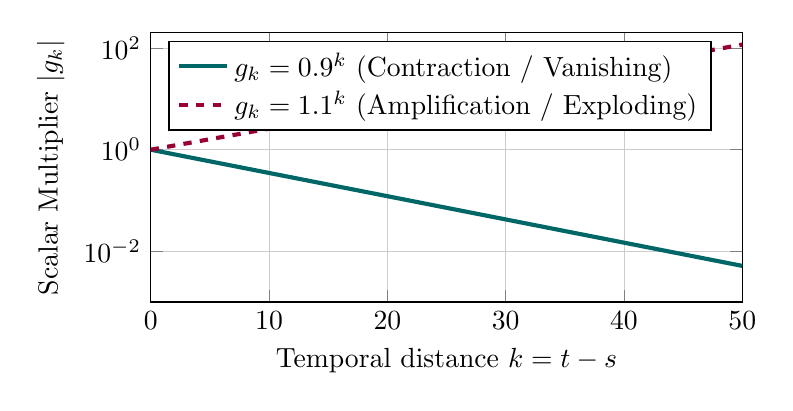
\begin{tikzpicture}
\begin{axis}[
    width=0.75\textwidth,
    height=5.0cm,
    ymode=log,
    xlabel={Temporal distance $k = t - s$},
    ylabel={Scalar Multiplier $|g_k|$},
    grid=both,
    grid style={line width=.1pt, draw=gray!20},
    major grid style={line width=.2pt, draw=gray!40},
    xmin=0, xmax=50,
    ymin=1e-3, ymax=2e2,
    legend pos=north west,
    legend cell align={left}
]
    \addplot[domain=0:50, samples=51, line width=1.5pt, teal!80!black] {0.9^x};
    \addlegendentry{$g_k = 0.9^k$ (Contraction / Vanishing)}
    
    \addplot[domain=0:50, samples=51, line width=1.5pt, dashed, purple!80!black] {1.1^x};
    \addlegendentry{$g_k = 1.1^k$ (Amplification / Exploding)}
\end{axis}
\end{tikzpicture}
\caption{Exponential contraction and growth of gradient magnitudes over temporal horizons.}
\end{figure}

\subsection{Gradient Norm Clipping \emph{(slides 84--86)}}
To prevent exploding gradients from destabilizing parameters during optimization, Pascanu et al.\ introduced global norm clipping:

\begin{algorithm}[Global Gradient Norm Clipping]
Given the unclipped global gradient vector $\mathbf{g} = \nabla_{\boldsymbol{\theta}} \mathcal{L}$ formed by concatenating all parameter gradients, and a predefined norm threshold $\tau > 0$:
\begin{equation}
    \mathbf{g}_{\text{clipped}} = \begin{cases}
        \mathbf{g}, & \text{if } \|\mathbf{g}\|_2 \le \tau, \\
        \dfrac{\tau}{\|\mathbf{g}\|_2} \mathbf{g}, & \text{if } \|\mathbf{g}\|_2 > \tau.
    \end{cases}
\end{equation}
Equivalently:
\begin{equation}
    \mathbf{g}_{\text{clipped}} = \min\left(1, \frac{\tau}{\|\mathbf{g}\|_2}\right) \mathbf{g}.
\end{equation}
\end{algorithm}

\begin{proposition}[Properties of Global Norm Clipping]
Norm clipping guarantees:
\begin{enumerate}
    \item Strict norm boundedness: $\|\mathbf{g}_{\text{clipped}}\|_2 \le \tau$.
    \item Directional fidelity: $\frac{\mathbf{g}_{\text{clipped}}}{\|\mathbf{g}_{\text{clipped}}\|_2} = \frac{\mathbf{g}}{\|\mathbf{g}\|_2}$ for all $\mathbf{g} \neq \mathbf{0}$.
    \item Bounded SGD step size: Under standard Stochastic Gradient Descent $\boldsymbol{\theta}^{(k+1)} = \boldsymbol{\theta}^{(k)} - \eta \mathbf{g}_{\text{clipped}}$, the parameter shift is strictly bounded: $\|\boldsymbol{\theta}^{(k+1)} - \boldsymbol{\theta}^{(k)}\|_2 \le \eta \tau$.
\end{enumerate}
\end{proposition}

\begin{figure}[htbp]
\centering
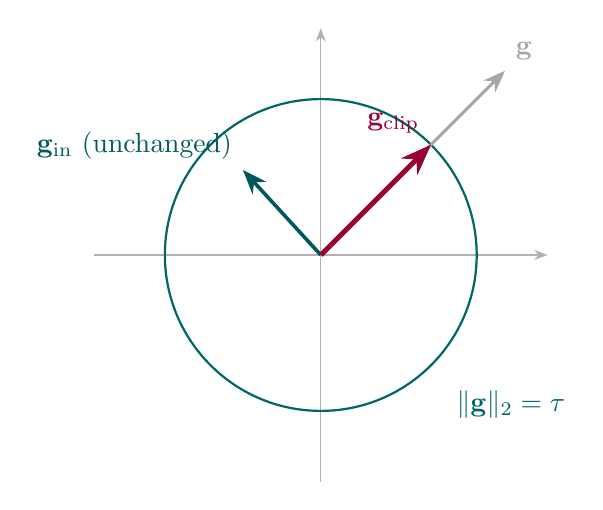
\begin{tikzpicture}[scale=0.9, >=Stealth]
    % Coordinate axes
    \draw[->, color=gray!60] (-3.2, 0) -- (3.2, 0);
    \draw[->, color=gray!60] (0, -3.2) -- (0, 3.2);
    
    % Clipping circle of radius tau
    \draw[thick, teal!80!black] (0, 0) circle (2.2cm);
    \node[teal!80!black, below right=1.6cm and 1.6cm of {(0,0)}] {$\|\mathbf{g}\|_2 = \tau$};
    
    % Small gradient (inside)
    \draw[->, line width=1.3pt, teal!70!black] (0, 0) -- (-1.1, 1.2) node[above left] {$\mathbf{g}_{\text{in}}$ (unchanged)};
    
    % Large gradient (outside) and clipped projection
    \draw[->, line width=1.1pt, gray!70] (0, 0) -- (2.6, 2.6) node[above right] {$\mathbf{g}$};
    \draw[->, line width=1.8pt, purple!80!black] (0, 0) -- (1.556, 1.556) node[above left] {$\mathbf{g}_{\text{clip}}$};
\end{tikzpicture}
\caption{Geometric visualization of global gradient norm clipping: vectors outside the hypersphere of radius $\tau$ are projected radially back onto the boundary, preserving direction.}
\end{figure}

\subsection{Truncated Backpropagation Through Time (TBPTT) \emph{(slide 87)}}
In full BPTT, computing gradients across a sequence of length $T$ requires storing all intermediate hidden activations $\mathbf{h}_1, \dots, \mathbf{h}_T$ in GPU/CPU memory, resulting in $\mathcal{O}(T)$ memory complexity per sequence. When $T$ is very large or infinite, full BPTT becomes physically intractable.

\begin{definition}[Truncated BPTT]
The sequence is split into manageable chunks of length $k_1$. Forward activations are propagated continuously across chunks to preserve stateful memory:
\begin{equation}
    \mathbf{h}_0^{(c+1)} = \mathbf{h}_{k_1}^{(c)}.
\end{equation}
However, during backpropagation, the computational autograd graph is \textbf{detached} at chunk boundaries:
\begin{equation}
    \frac{\partial \mathbf{h}_0^{(c+1)}}{\partial \boldsymbol{\theta}} \leftarrow \mathbf{0}.
\end{equation}
Adjoint errors $\boldsymbol{\delta}_t$ propagate backward at most $k_1$ steps, bounding memory and computation to $\mathcal{O}(k_1)$ while allowing forward dynamics to integrate long histories.
\end{definition}

% =============================================================
\section{Summary \& Comparative Synthesis}
% =============================================================

\subsection{Architectural Paradigm Comparison}
To consolidate the foundational paradigms covered throughout this lecture, Table~\ref{tab:comparison} details their structural, operational, and computational tradeoffs.

\begin{table}[htbp]
\centering
\small
\begin{tabular}{@{}p{3.2cm}p{3.6cm}p{4.2cm}p{3.8cm}@{}}
\toprule
\textbf{Model Class} & \textbf{Memory Representation} & \textbf{Advantages} & \textbf{Limitations} \\ \midrule
\textbf{Classical Linear} \newline ($\operatorname{AR}, \operatorname{ARMA}, \operatorname{ARIMA}$) & Explicit lag coefficients over raw past values and innovations. & Globally optimal convex estimation (Yule-Walker, MLE); statistical interpretability. & Restricted to linear dynamics; brittle under non-Gaussian multimodal regimes. \\ \addlinespace
\textbf{Buffered MLP} & Tapped delay line concatenated into static vector $\mathbf{v}_t \in \mathbb{R}^{pd}$. & Stable feedforward training; cannot suffer from vanishing/exploding recurrent gradients. & Strictly truncated context $p$; parameters scale with window size; exposure bias in rollouts. \\ \addlinespace
\textbf{Vanilla Elman RNN} & Recursively updated hidden state $\mathbf{h}_t = \phi(\mathbf{W}_x \mathbf{x}_t + \mathbf{W}_h \mathbf{h}_{t-1} + \mathbf{b})$. & Arbitrary-length temporal capacity; parameter count independent of sequence length $T$. & Severe vanishing/exploding gradients; difficulty capturing long-term dependencies; sequential computation prevents full temporal parallelization. \\ \bottomrule
\end{tabular}
\caption{Systematic comparison of sequential modeling paradigms.}
\label{tab:comparison}
\end{table}

\subsection{Empirical One-Step Error Floor and the Irreducible Innovation Variance \emph{(slide 94)}}
When assessing time-series forecasting models, empirical Mean Squared Error must always be evaluated relative to the fundamental stochastic lower bound established by the innovation noise.

\begin{proposition}[Bayes Risk Error Floor in Additive Innovation Models]
Consider an observed stochastic process governed by $x_t = \mu(x_{1:t-1}) + \epsilon_t$, where $\epsilon_t \sim \text{i.i.d. } \mathcal{N}(0, \sigma_\epsilon^2)$. For any causal estimator $\hat{x}_t = g(x_{1:t-1})$, the expected one-step prediction MSE is bounded below by the innovation variance:
\begin{equation}
    \mathbb{E}\left[(x_t - \hat{x}_t)^2\right] = \mathbb{E}\left[(\mu(x_{1:t-1}) - \hat{x}_t)^2\right] + \sigma_\epsilon^2 \ge \sigma_\epsilon^2.
\end{equation}
\end{proposition}

\slideimageplaceholder{92, 93 \& 94}{Comparative test trajectories for Buffered MLP vs. Vanilla RNN on the synthetic noisy sinusoid benchmark, highlighting how both converge near the irreducible error floor $\sigma_\epsilon^2 = (0.2)^2 = 0.04$ on one-step prediction, but diverge significantly over recursive multi-step rollouts.}

\subsection{Key Takeaways}
\begin{itemize}
    \item \textbf{Sequence Representation vs. Statefulness:} Sequence data can be processed by static feedforward networks using external tapped delay lines, or by recurrent models maintaining internal dynamical hidden states. Neither paradigm universally dominates; strong feedforward baselines (e.g., linear models, DLinear, TSMixer) often outperform un-gated recurrent nets on long horizons.
    \item \textbf{Recurrent Inductive Bias:} An Elman RNN ties parameter tensors across all temporal positions ($N_{\text{par}}$ is independent of sequence length $T$), compressing history $\mathbf{x}_{1:t}$ into an evolving hidden vector $\mathbf{h}_t \in \mathbb{R}^m$.
    \item \textbf{The Vanishing/Exploding Gradient Dilemma:} BPTT computes exact shared-parameter gradients via reverse-time chain rule products $\prod_{j=s+1}^t \mathbf{J}_j$. Because $\mathbf{J}_j = \operatorname{diag}(\phi'(\mathbf{a}_j))\mathbf{W}_h$, these matrix products decay or grow exponentially over long time horizons, severely hindering the learning of distant dependencies.
    \item \textbf{Practical Stabilization:} Gradient norm clipping radially bounds update steps to eliminate catastrophic explosion; truncated BPTT detaches backpropagation graphs to bound compute/memory to $\mathcal{O}(k_1)$; and learnable gating structures (such as LSTMs and GRUs, explored in subsequent lectures) are required to systematically combat vanishing gradients.
\end{itemize}

\end{document}